\section{Diagramme de classe}

\begin{figure}[H]
  \center
  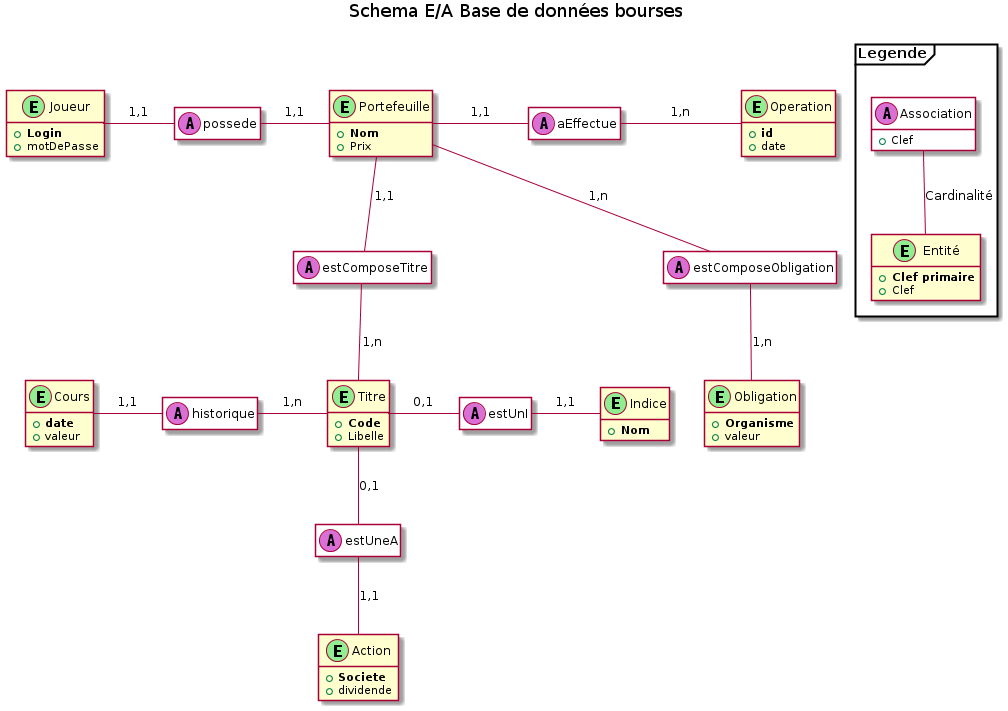
\includegraphics[scale=0.25]{../graph/DiagrammeEntiteAssociation.png} \\
  \caption{Modélisation de notre base de données}
\end{figure}

Ce schéma représente la modélisation de notre base de données. La modélisation est la même que pour la partie modèle de notre projet. Le joueur possède un portefeuille qui comporte lui même soit des titres soit des obligations. Le portefeuille possède également sa liste d'opérations dans une nouvelle table. Nous avons une table qui contient l'ensemble des titres disponibles que ce soit indice ou action, une table qui contient l'ensemble des obligations. Nous avons également une table qui contient l'historique pour un titre. 